\documentclass[12pt]{amsart}

\theoremstyle{plain}
\newtheorem{theorem}{Theorem}
\newtheorem{lemma}[theorem]{Lemma} 
\newtheorem{conjecture}[theorem]{Conjecture} 
\newtheorem{corollary}[theorem]{Corollary}
\newtheorem{proposition}[theorem]{Proposition}
\theoremstyle{definition}
\newtheorem{definition}[theorem]{Definition}
\newtheorem*{question}{Question}

\usepackage{fullpage,hyperref,url}
\usepackage[pdftex]{graphicx}

\title{Quintic Spectrahedra}
\author{Jacob Emmert-Aronson}
\author{Moor Xu}
\date{May 7, 2014}
\begin{document} 
\maketitle

\emph{Spectrahedra} of degree $n$ in $\mathbb{R}^k$ are convex bodies
given by $k$-dimensional affine slices of the cone of $n \times n$
positive semidefinite matrices.  They arise as feasible domains in
semidefinite programming and each is described by a linear matrix
inequality. We will work with spectrahedra in $\mathbb R^3$.

\begin{definition} 
	A \emph{spectrahedron} of degree $n$ in $\mathbb R^3$ is a convex body
	of the form 
	\[ 
		S = \left\{
		(x,y,z) \mid Ax + By + Cz + D \text{ is positive semidefinite} \right\}
	\] 
	where $A$, $B$, $C$, $D$ are real symmetric $n\times n$ matrices.
\end{definition} 

\bigskip
%\vspace\baselineskip

\begin{center}
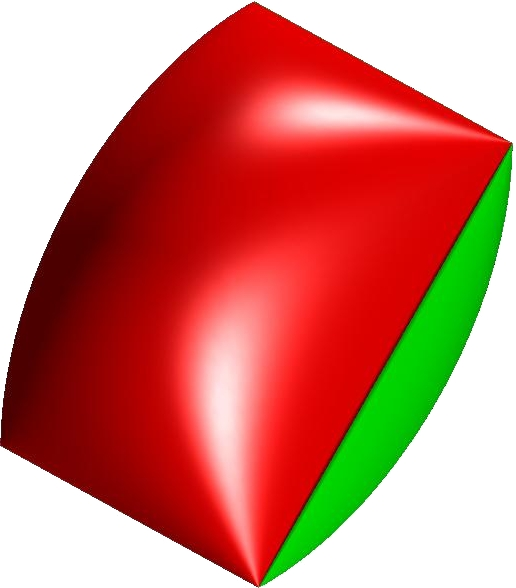
\includegraphics[scale=.15]{pillow.jpg}
%\vspace\baselineskip
\bigskip

{\small
\emph{The pillow}: the spectrahedron
$
\begin{pmatrix}
  1&x&0&x\\
  x&1&y&0\\
  0&y&1&z\\
  x&0&z&1
\end{pmatrix}
\succeq 0\text.$  Here $k=3,\, n=4$.}
\end{center}
%\vspace\baselineskip
\bigskip

Because the cost function of an SDP is linear, the optimal point
always lies on the surface.  One interesting and practically useful
question is the likelihood for the result of an optimization to be a
node, one of the corner points seen when visualizing the
spectrahedron.  A generic matrix represented by a point on the surface
of the spectrahedron has rank $n-1$, while the matrix at a node
typically has rank $n-2$.  This low-rank property of nodes often
translates to easier computation.

To better understand the nodal structure of spectrahedra, we work with the
notion of a symmetroid.
\begin{definition} 
	The \emph{symmetroid} $S$ of degree $n$ is a surface defined by 
	\[ 
		\det (Ax + By + Cz + D) = 0
	\] 
	where $A$, $B$, $C$, $D$ are $n\times n$ matrices.
\end{definition} 
A spectrahedron can be thought of as a component of the symmetroid.
To compute the nodes of a spectrahedron, we compute the nodes of the
symmetroid, and see how many lie on the spectrahedron.

\begin{proposition} 
	Generically, a symmetroid $S$ of degree $n$ has $\binom{n+1}3$ nodes.
\end{proposition} 

\begin{question} 
How many nodes can be real? How many nodes can lie on the spectrahedron?
\end{question} 

These questions have been answered in the quartic case. 
\cite{OKSV} classifies the number of nodes that quartic spectrahedra can have. 
\begin{theorem}\label{quartic}
	There exists a quartic spectrahedron with $\sigma$ nodes on its boundary and
	$\rho$ real nodes in its symmetroid if and only if $0 \le \sigma \le \rho$,
	both are even, and $2 \le \rho \le 10$.
\end{theorem} 
This means that there are 20 types of quartic spectrahedra, each with its own
$(\rho, \sigma)$ node count. 

We studied the nodal structure of quintic spectrahedra in hopes of obtaining an
analogous result.

To carry this out, we generated random spectrahedra and computed
the positions of nodes, while also running multiple optimization
problems on each.  Jacob Emmert-Aronson and Joe Kileel wrote much of
the code to carry this out last semester.  
We had used Singular
to determine locations of nodes through a Gr\"obner basis algorithm;
due to apparent numeric instabilities, however, this misidentified
nodes in certain edge cases.  We have replaced this with the
homotopy algorithms implemented in Bertini, which have produced more
reliable results.  

More specifically, here is what we did:
\begin{itemize}
	\item Generate matrices $A$, $B$, $C$, $D$.
	\item Use Bertini to compute the 20 complex nodes.
	\item Count the number of real nodes.
	\item For each real node, check if it lies on the spectrahedron. (A node
		lies on the spectrahedron if its eigenvalues have the same sign.)
\end{itemize}

DISCUSS HOW TO GENERATE MATRICES

%We are now generating a new data set to determine possible node counts with
%relative frequencies, and other properties which may be of interest.  After
%generating 6723 random quintic spectrahedra and computing their nodes, we have
%observed the following behavior. Here, $\sigma$ is the number of nodes on the
%boundary of the spectrahedra, $\rho$ is the number of real nodes in its
%symmetroid, and $p$ is the probability of observing these node counts upon
%generating a random quintic spectrahedron. (Some node counts occurred with
%very low probability.)

%\begin{center}
%\begin{tabular}{| l | l | l |} 
%	$\sigma$ & $\rho$ & $p$ \\ \hline
%	0 & 4 & 0.002    \\
%	0 & 6 & 0.002    \\
%	0 & 8 & low    \\
%	0 & 10 & low    \\
%	2 & 2 & low    \\
%	2 & 4 & 0.010    \\
%	2 & 6 & 0.061    \\
%	2 & 8 & 0.075    \\
%	2 & 10 & 0.028    \\
%	2 & 12 & 0.005    \\
%	2 & 14 & 0.001    \\
%	4 & 4 & low    \\
%	4 & 6 & 0.023    \\
%	4 & 8 & 0.153    \\
%	4 & 10 & 0.236    \\
%	4 & 12 & 0.096    \\
%	4 & 14 & 0.021    \\
%	4 & 16 & 0.003    \\
%	6 & 6 & low    \\
%	6 & 8 & 0.009    \\
%	6 & 10 & 0.065    \\
%	6 & 12 & 0.114    \\
%	6 & 14 & 0.056    \\
%	6 & 16 & 0.013    \\
%	6 & 18 & 0.001    \\
%	8 & 10 & 0.001    \\
%	8 & 12 & 0.005    \\
%	8 & 14 & 0.011    \\ \hline
%\end{tabular} 
%\end{center}
DATA GOES HERE

%We believe that with more data, we will see more types of quintic spectrahedra,
%and we conjecture that a result analogous to Theorem \ref{quartic} holds in the
%quintic case. This requires some further study.

DISCUSS FURTHER IMPROVEMENTS

APPENDIX WITH A GALLERY OF SPECTRAHEDRA?


%%%%%%%%%%%%%%%%%%%%%%%
\bibliographystyle{amsplain}
\bibliography{references}
\nocite{*}

\end{document} 


